\begin{definition}[Parametrização]
  Seja $V\subseteq\mathbb{R}^{n}$. Uma \textbf{parametrização} de classe $C^{k}$ de $V$ é um homomorfismo $\phi:V_0\to V$, onde $V_0\subseteq \mathbb{R}^{m}$ é aberto e
  \begin{itemize}
    \item $\phi$ é injetivo.
    \item $\phi\in C^{k}$.
    \item $\phi^{\prime}(x):\mathbb{R}^{m}\to\mathbb{R}^{n}$ é injetiva para todo $x\in\mathbb{R}^{m}$ ($\phi$ é uma imersão).
  \end{itemize}
\end{definition}
\begin{note}
  Toda parametrização é um difeomorfismo sobre sua imágem (Dica: Use o teorema da aplicação inversa).
\end{note}
\begin{definition}[Superficie]
  Um conjunto $M\subseteq \mathbb{R}^{n}$ é uma superficie de dimensão $m$ e classe $C^{k}$ se para todo $p\in M$ existe um aberto $U\subseteq\mathbb{R}^{n}$ tal que $V=U\cap M$, admite uma parametrização $\phi:V_0\to V$ $C^{k}$ com $V_0\subseteq\mathbb{R}^{m}$ aberto.
  \begin{center}
    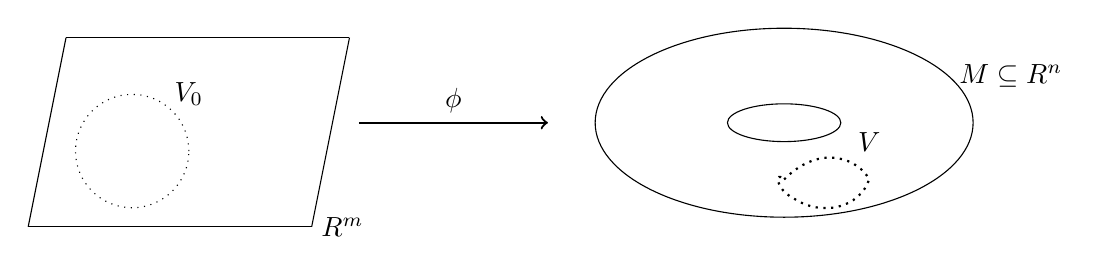
\begin{tikzpicture}[scale=1.2]

% --- Dominio en R^2 ---
\begin{scope}
  \draw[-] (0,0.4) -- (3,0.4) node[right] {$\mathbb{R}^{m}$};
  \draw[-] (0.4,2.4) -- (3.4,2.4);
  \draw[-] (3,0.4) -- (3.4,2.4);
  \draw[-] (0,0.4) -- (0.4,2.4);

  % Abierto (rectángulo)
  \draw[dotted] (1.1,1.2) circle (0.6);

  \node at (1.7,1.8) {$V_0$};
\end{scope}

% Flecha phi
\draw[->, thick] (3.5,1.5) -- (5.5,1.5) node[midway, above] {$\phi$};

% --- Toro (aproximación 2D) ---
\begin{scope}[xshift=8cm]

  % Contorno exterior (elipse grande)
  \draw (0,1.5) ellipse (2 and 1);

  % Agujero interior
  \draw (0,1.5) ellipse (0.6 and 0.2);

\draw[dotted, thick]
  (0,0.9)
  .. controls (0.4,1.3) and (0.8,1.1) ..
  (0.9,0.9)
  .. controls (0.8,0.6) and (0.4,0.5) ..
  (0.1,0.7)
  .. controls (-0.1,0.8) and (-0.1,1) ..
  cycle;

\node at (0.9,1.3) {$V$};
\node at (2.4,2) {$M\subseteq \mathbb{R}^{n}$};
\end{scope}
\end{tikzpicture}

      
  \end{center}
\end{definition}
\begin{note}
  \phantom{X}
  \begin{itemize}
    \item Se $\dim M=1$, então $M$ é uma curva.
    \item Se $\dim M=n-1$, então $M$ é uma hipersuperfície.
    \item A codimensão de $M$ é $n-m$. 
  \end{itemize}
\end{note}
\begin{example}
  Todo aberto $U\subseteq\mathbb{R}^{n}$ é uma superfície de dimensão $n$ e de classe $C^{\infty}$, tome $\phi=Id_{\mathbb{R}^{n}}$.
\end{example}
\begin{example}
  Se para cada ponto $p\in M$ tem uma vizinhançã $Z\subseteq\mathbb{R}^{n}$ tal que $Z\cap M$ é uma superfície de dimensão $m$, então $M$ é uma superfície de dimensão $m$. 
\end{example}
\begin{example}
  $f:U\to\mathbb{R}^{n}$ $C^{k}$ com $U\subseteq \mathbb{R}^{m}$ aberto, logo o gráfico de $f$
  \begin{align*}
    M=\{(x,f(x))\in\mathbb{R}^{m+n}:x\in U\}
  \end{align*}
  é uma superfície de dimensão $m$ e de classe $C^{k}$ com $\phi(x)=(x,f(x))$. 
\end{example}
\begin{note}[Espaço Tangente]
  Seja $M$ uma superfície com $\dim M=m$ e $p\in M$, então as seguintes afirmações são equivalentes
  \begin{enumerate}
    \item Seja $\phi:V_0\to V$ parametrização com $\phi(a)=p$, então
      \begin{align*}
        T_pM=\phi^{\prime}(a)\cdot \mathbb{R}^{m}=\{\phi^{\prime}(a)\cdot :v\in\mathbb{R}^{m}\}.
      \end{align*}
      Note que $T_pM$ é um espaço vetorial de $\mathbb{R}^{n}$ de dimensão $m$.
    \item Seja $\gamma:(-\epsilon,\epsilon)\to M$ difeomorfismo com $\gamma(0)=p$, então
      \begin{align*}
        T_p M=\{\gamma^{\prime}(0):\gamma\text{ é uma curva em $M$ com }\gamma(0)=p\}
      \end{align*}
  \end{enumerate}
\end{note}
\begin{definition}[Diferenciabilidade na superfície]
  Seja $M\subseteq\mathbb{R}^{n}$ $C^{k}$ com $k\geq 1$.\\
  Dezimos que $f:M\to\mathbb{R}^{r}$ é \textbf{diferenciável} no ponto $p\in M$ quando existe uma parametrização $C^{k}$ $\phi:V_0\to V$ tal que $f\circ \phi:V_0\to\mathbb{R}^{r}$ é diferenciável em $a=\phi^{-1}(p)$.
  \begin{center}
    \input{images/diferenciabilidadenasuperficie}  
  \end{center}
\end{definition}
\begin{note}
  Note que se $\Psi$ é outra parametrização, você tem $f\circ \Psi=f\circ \phi\circ \phi^{-1}\circ \Psi$, pelo que a derivada na superfície queda bém definida. 
\end{note}
\begin{definition}[$f$ de classe $C^{i}$]
  Seja $f:M\to\mathbb{R}^{r}$, definida numa superfície $M$ de classe $C^{k}$, dizemos que $f$ é de classe $C^{i}$ quando para cada ponto $p\in M$ existe uma parametrização $\phi:V_0\to V\subseteq M$ com $p\in M$ e $\phi\in C^{k}$ tal que $f\circ \phi:V_0\to\mathbb{R}^{r}$ é de classe $C^{i}$ no aberto $V_0\subseteq \mathbb{R}^{m}$. 
\end{definition}
\begin{note}
  Note que como $\phi\in C^{k}$, se $f\in C^{i}$, então $i\leq k$.  
\end{note}
\begin{note}
  Se $f:M\to\mathbb{R}^{r}$ é diferenciável no ponto $p\in M$, então sua derivada é uma transformação linear $f^{\prime}(p):T_pM\to\mathbb{R}^{r}$ definida do seguinte modo, se tomamos uma parametrização $\phi:V_0\to V$ com $p=\phi(a)$. Dado $v\in T_pM$ temos que $v=\phi^{\prime}(a)\cdot v_0$ para algúm $v_0\in \mathbb{R}^{m}$. Definimos
  \begin{align*}
    f^{\prime}(p)\cdot v= (f\circ \phi)^{\prime}(a)\cdot v_0.
  \end{align*}
  \textcolor{red}{Ela está bem definida, verificar!}
\end{note}
\begin{definition}[Diferenciabilidade entre superfícies]
  Seja $M\subseteq \mathbb{R}^{n}$ uma superfície de classe $C^{k}$ e $N\subseteq \mathbb{R}^{r}$ outra superfície de classe $C^{k}$ e a aplicação $f:M\to \mathbb{R}^{r}$ é uma aplicação diferenciável no ponto $p\in M$ é tal que $f(M)\subseteq N$, diremos que $f:M\to N$ é diferenciável no ponto $p$.
  \begin{center}
    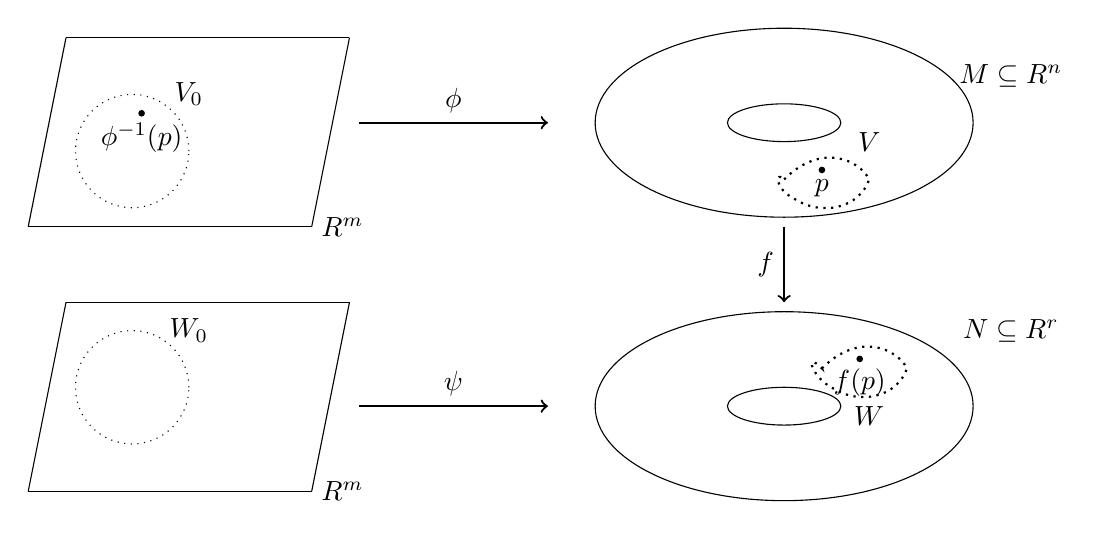
\begin{tikzpicture}[scale=1.2]

% --- Dominio en R^2 ---
\begin{scope}
  \draw[-] (0,0.4) -- (3,0.4) node[right] {$\mathbb{R}^{m}$};
  \draw[-] (0.4,2.4) -- (3.4,2.4);
  \draw[-] (3,0.4) -- (3.4,2.4);
  \draw[-] (0,0.4) -- (0.4,2.4);

  % Abierto (rectángulo)
  \draw[dotted] (1.1,1.2) circle (0.6);

  \node at (1.7,1.8) {$V_0$};
\end{scope}

% Flecha phi
\draw[->, thick] (3.5,1.5) -- (5.5,1.5) node[midway, above] {$\phi$};

% --- Toro (aproximación 2D) ---
\begin{scope}[xshift=8cm]

  % Contorno exterior (elipse grande)
  \draw (0,1.5) ellipse (2 and 1);

  % Agujero interior
  \draw (0,1.5) ellipse (0.6 and 0.2);

\draw[dotted, thick]
  (0,0.9)
  .. controls (0.4,1.3) and (0.8,1.1) ..
  (0.9,0.9)
  .. controls (0.8,0.6) and (0.4,0.5) ..
  (0.1,0.7)
  .. controls (-0.1,0.8) and (-0.1,1) ..
  cycle;

\node at (0.9,1.3) {$V$};
\node at (2.4,2) {$M\subseteq \mathbb{R}^{n}$};
\end{scope}

% Segunda

\begin{scope}
  \draw[-] (0,-2.4) -- (3,-2.4) node[right] {$\mathbb{R}^{m}$};
  \draw[-] (0.4,-0.4) -- (3.4,-0.4);
  \draw[-] (3,-2.4) -- (3.4,-0.4);
  \draw[-] (0,-2.4) -- (0.4,-0.4);

  % Abierto (rectángulo)
  \draw[dotted] (1.1,-1.3) circle (0.6);

  \node at (1.7,-0.7) {$W_0$};
\end{scope}

% Flecha phi
\draw[->, thick] (3.5,-1.5) -- (5.5,-1.5) node[midway, above] {$\psi$};

% --- Toro (aproximación 2D) ---
\begin{scope}[xshift=8cm]

  % Contorno exterior (elipse grande)
  \draw (0,-1.5) ellipse (2 and 1);

  % Agujero interior
  \draw (0,-1.5) ellipse (0.6 and 0.2);

\draw[dotted, thick]
  (0.4,-1.1)
  .. controls (0.8,-0.7) and (1.2,-0.9) ..
  (1.3,-1.1)
  .. controls (1.2,-1.4) and (0.8,-1.5) ..
  (0.5,-1.3)
  .. controls (0.3,-1.2) and (0.2,-0.9) ..
  cycle;

\node at (0.9,-1.6) {$W$};
\node at (2.4,-0.7) {$N\subseteq \mathbb{R}^{r}$};
\end{scope}

\draw[->, thick] (8,0.4) -- (8,-0.4) node[midway, left] {$f$};

\fill (1.2,1.6) circle (1pt);
  \node[below] at (1.2,1.6) {$\phi^{-1}(p)$}; 

\fill (8.4,1) circle (1pt);
  \node[below] at (8.4,1) {$p$}; 

\fill (8.8,-1) circle (1pt);
  \node[below] at (8.8,-1) {$f(p)$}; 
\end{tikzpicture}
  
  \end{center}
\end{definition}
\begin{proposition}[Regra da cadeia]
  Se $f:M\to N$, $g:N\to\mathbb{R}^{s}$ diferenciáveis, então
  \begin{align*}
    (g\circ f)^{\prime}(p)=g^{\prime}(f(p))\cdot f^{\prime}(p).
  \end{align*}
\end{proposition}
\begin{definition}[Ponto regular]
  Seja $f:U\to\mathbb{R}^{n-m}$ de classe $C^{k}$, com $U\subseteq \mathbb{R}^{n}$ aberto. Um ponto $c\in\mathbb{R}^{n-m}$ é \textbf{ponto regular} se para todo $x\in f^{-1}(c)$, a derivada $f^{\prime}(x):\mathbb{R}^{n}\to\mathbb{R}^{m}$ é sobrejetiva. 
\end{definition}
\begin{theorem}
  Seja $f:U\to\mathbb{R}^{n-m}$ $C^{k}$ e $U\subseteq\mathbb{R}^{n}$ aberto. Se $c\in \mathbb{R}^{n-m}$ é valor regular, então $M=f^{-1}(c)$ é uma superfície de dimensão e classe $C^{k}$. Além disso, para cada $p\in M$
  \begin{align*}
    T_pM=\Ker f^{\prime}(p).
  \end{align*}
\end{theorem}
\begin{proof} 
  Pelo teorema do função implícita, para cada $p\in M$ existe um aberto $Z\subseteq \mathbb{R}^{n}$ tal que $Z\cap M$ é o gráfico de uma função de classe $C^{k}$ de $\mathbb{R}^{n}$ em $\mathbb{R}^{n-m}$. Logo, $Z\cap M$ é uma superfície de dimensão $m$. Como isso vale para todo ponto $p\in M$, então $M$ é uma superfície.
  \begin{itemize}
    \item Se $\gamma:I\to M$ é uma curva em $M$ com $r(o)=p$, então temos que $f(\gamma(0))=c$.\\
      Derivando temos que $f^{\prime}(p)\cdot \gamma^{\prime}(0)=0$, então $r^{\prime}(0)\in \Ker f^{\prime}(p)$. Logo ambos tem a mesma dimensão, ja que
      \begin{align*}
        \dim \Ker f^{\prime}(p)+\dim\Img f^{\prime}(p)=n.
      \end{align*}
      Mas como $\dim\Img f^{\prime}(p)=n-m$, temos que $\dim\Ker f^{\prime}(p)=m$.
  \end{itemize}
\end{proof}
\begin{definition}[Mudançã de parametrização]
  Sejam $\phi:V_0\to V$ e $\varphi:W_0\to W$ parametrizações em $M$ com $V\cap W\neq \emptyset$. A aplicação $\varphi\circ\phi:\phi^{-1}(V\cap W)\to\varphi^{-1}(V\cap W)$ é chamada \textbf{mudançã de parametrizações}. 
\end{definition}
\begin{theorem}
  Seja $\phi:V_0\to V$ parametrização em $M$. Para cada $p=\phi(x_0)\in V$, existe uma projeção $\pi:\mathbb{R}^{n}\to\mathbb{R}^{m}$ tal que $\pi\circ\phi$ é um difeomorfismo de uma vizinhança $Z_0\subseteq V_0$ sobre um aberto de $\mathbb{R}^{m}$
  \begin{equation}\label{eq:projecao3.12}
    \pi(x_1,\cdots,x_n)=(x_{i_1},x_{i_{2}},\cdots,x_{i_m}).
  \end{equation}
\end{theorem}
\begin{proof} 
  A matriz Jacobiana de $\phi$ em $x_0$ tem $m$ linhas linearmente independentes. Com essas linhas defina $\pi$ da forma do \eqref{eq:projecao3.12} (da mesma maneira que no lema \ref{lema:3.11-2teoremadoposto}). Logo $\pi\circ\phi$ tem derivada invertível nesse ponto, logo pelo teorema da aplicação inversa, é um difeomorfismo local. 
\end{proof}
\begin{note}
  \phantom{xxx}
  \begin{itemize}
    \item Toda superfície é localmente o gráfico de uma função de classe $C^{k}$.
    \item $f:V_0\to\mathbb{R}^{n}$ $C^{k}$ e sua imagem esta contida em $W\subseteq M$ parametrizado por $\psi$, então $\psi^{-1}\circ f$ é $C^{k}$.
    \item $\psi^{-1}\circ \phi$ é difeomorfismo de classe $C^{k}$. 
  \end{itemize}
\end{note}
\begin{theorem}[Teorema da aplicação inversa entre superfícies]
  Sejam $M\subseteq\mathbb{R}^{n}$, $N\subseteq\mathbb{R}^{s}$ superfícies de classe $C^{k}$ com ($k\geq 1$) e $f:M\to N$ diferenciável. Se $p\in M$ é tal que $f^{\prime}(p):T_{p}M\to T_{f(p)}N$ é um isomorfismo, então existem vizinhanças $U\subseteq M$ de $p$ e $V\subseteq N$ de $f(p)$ tais que $f\big|_{U}:U\to V$ é um difeomorfismo. 
\end{theorem}
\begin{proof} 
  \phantom{xxx}
  \begin{itemize}
    \item $f^{\prime}(p)$ é bijetiva, então $\dim M=\dim N=m$.
    \item Tome parametrizações $\phi:Z_0\to Z\subseteq M$ com $\phi(a)=p$ e $\psi:W_0\to W\subseteq N$ com $\psi(b)=f(b)$.
    \item Considere $F:\psi^{-1}\circ f\circ \phi:Z_0\to W_0$ que é $C^{k}$ e note que
      \begin{align*}
        F^{\prime}(a)=(\psi^{-1})(f(p))\cdot f^{\prime}(p)\cdot\phi^{\prime}(a).
      \end{align*}
      Como $\psi$ e $\phi$ são difeomorfismos, temos que $F$ é isomorfismo e temos que $F^{\prime}(a)$ é invertível.
    \item Pelo teorema da aplicação inversa em $\mathbb{R}^{m}$, $F$ é difeomorfismo local, logo existem abertos vizinhanças abertas $U_0\subseteq Z_0$ de $a$ e $V_0\subseteq W$ de $b$ tais que $F\big|_{U_0}:U_0\to V_0$ é difeomorfismo.
    \item Defina $U=\phi(U_0)$ e $V=\psi(V_0)$. Então $f\big|_{U}=\psi\circ F\circ \phi:U\to V$ é difeomorfismo. 
  \end{itemize}
\end{proof}
